\documentclass[../main.tex]{subfiles}

\begin{document}

We first compare the results of with the generic one dimensional bootstrap particle filter of \tofix{Section X} and the drift-corrected particle filter described in \autoref{eq:2__2__1__drift_corrected_simple_PF}. 

To compare the results of both particle filtering methods, we use a dataset consisting of 60 minutes of high frequency tick data for the EUR/USD currency pair from the 16th of October 2019, totalling 4196 discrete price observations. 

Figure \ref{fig:4__1__1__bootstrap_PF} gives both the observed and inferred returns and price process for the simple bootstrap particle filter. We can clearly see the effectiveness of the noise removal in the inferred returns process. However, we note that the inferred price process suffers greatly from drift. Small errors in the inference of the returns process are compounded, leading to the inferred price process deviating from the observed price. 

This causes the poor inference results when the generic particle filter is used to infer the underlying price process of the simulated signal in Figure \ref{fig:4__1__comparison_price}.

\begin{figure}[h!]
	\centering
	\subfloat[Inferred Returns Process \label{fig:4__1__1__bootstrap_naiive}]{
		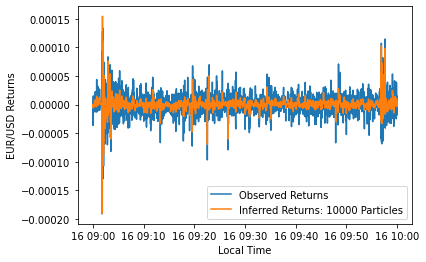
\includegraphics[height=4.5cm]{../plots/4__1__1__bootstrap_naiive.png}}
	\qquad
	\subfloat[Inferred Price Process \label{fig:4__1__1__bootstrap_naiive_price}]{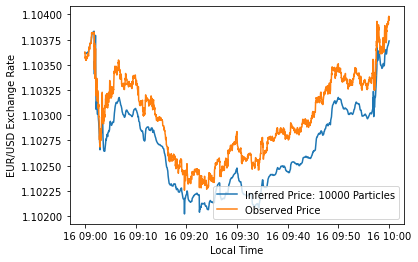
\includegraphics[height=4.5cm]{../plots/4__1__1__bootstrap_naiive_price.png}}
	\caption{Simple Bootstrap Particle Filter, $N = 10000$ particles}
	\label{fig:4__1__1__bootstrap_PF}
\end{figure}

The drift-corrected particle filter attempts to correct for price drift in the system by using numerical integration to obtain an estimate of the current inferred value of the price process at every time step. 

Figure \ref{fig:4__1__1__drift_corrected} gives both the observed and inferred returns and price process for the drift-corrected particle filter. We note qualitatively that the inferred returns process shows much greater noise reduction, and the inferred price process no longer suffers from price drift. 

\begin{figure}[h!]
	\centering
	\subfloat[Inferred Returns Process \label{fig:4__1__1__drift_corrected}]{
		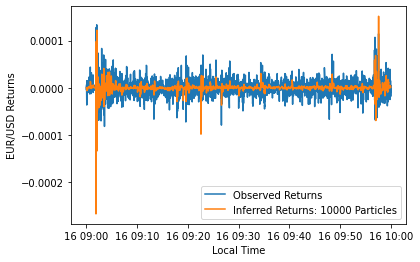
\includegraphics[height=4.5cm]{../plots/4__1__1__drift_corrected.png}}
	\qquad
	\subfloat[Inferred Price Process \label{fig:4__1__1__drift_corrected_price}]{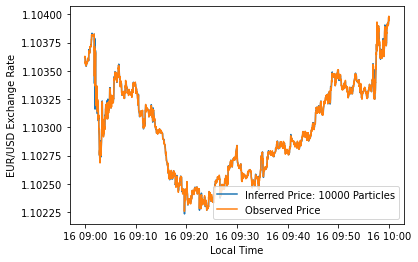
\includegraphics[height=4.5cm]{../plots/4__1__1__drift_corrected_price.png}}
	\caption{Drift-Corrected Particle Filter, $N = 10000$ particles}
	\label{fig:4__1__1__drift_corrected_PF}
\end{figure}

\textbf{Varying $N$}

Figure \ref{fig:4__1__1__boostrap_comparison} shows how the performance of the 2 bootstrap particles filters vary as the number of particles, $N$ is changed. Here, we apply  between the ground truth underlying price and return states from simulated data and the inferred underlying price and return states from the particle filters. This allows us to examine how well the particle filter tracks the actual underlying state.

\begin{figure}[h!]
	\centering
	\subfloat[RMSE of price($x_1$) state \label{fig:4__1__1__bootstrap_comparison_rmse_price}]{
		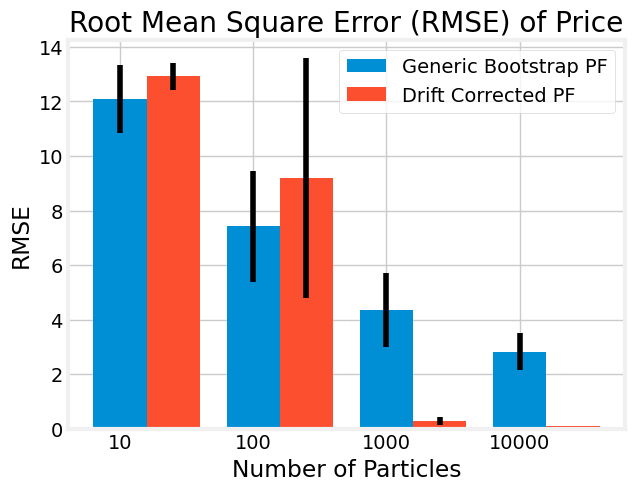
\includegraphics[height=4.5cm]{../plots/4__1__1__bootstrap_comparison_rmse_price.png}}
	\qquad
	\subfloat[RMSE of returns($x_2$)  state \label{fig:4__1__1__bootstrap_comparison_rmse_returns}]{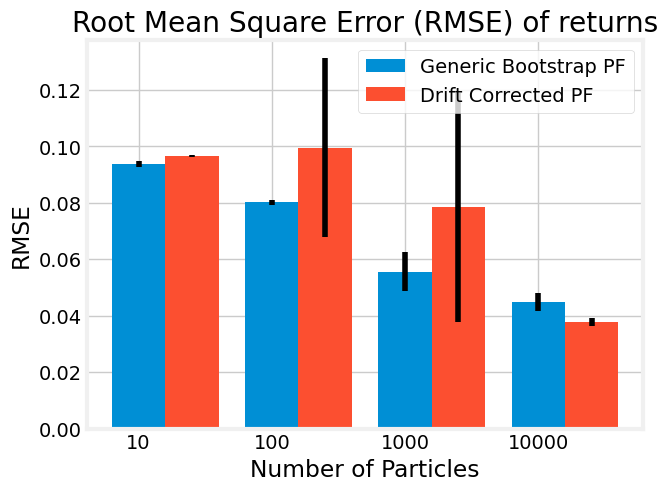
\includegraphics[height=4.5cm]{../plots/4__1__1__bootstrap_comparison_rmse_returns.png}}

	\qquad
	\subfloat[BPE of returns($x_2$)  state \label{fig:4__1__1__bootstrap_comparison_bpe_returns}]{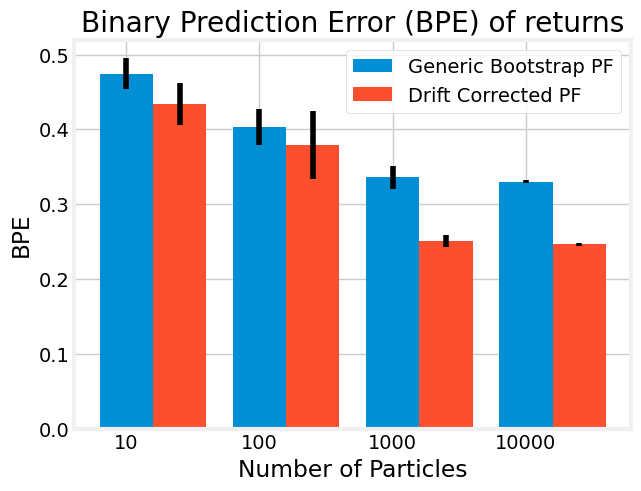
\includegraphics[height=4.5cm]{../plots/4__1__1__bootstrap_comparison_bpe_returns.png}}
	\caption{Comparison of inference performance between the 2 bootstrap particle filters as $N$ varies}
	\label{fig:4__1__1__boostrap_comparison}
\end{figure}

Both the generic bootstrap particle filter and the drift-corrected particle filter are both very sensitive to sample impoverishment in the same manner as described in \autoref{sec:inference_RBPF}. 

For low $N$ and large $y_k - \bvec{CA}\bvec{x}_{k-1}^{(i)}$, the samples of $\bvec{x}_k$ obtained from the particle filter proposal distribution are likely to have very low acceptance weights, resulting in a lack of particles with effective weights. If there are no particles with effective weights generated by the particle filter, the tracking performance of the particle filter can be severely diminished. The larger the observed price outlier ($y_k - \bvec{CA}\bvec{x}_{k-1}^{(i)}$) and the lower the number of particles $N$, the greater the impact of this problem. 

Thus, we expect the performance of the bootstrap particle filters to fall rapidly as the number of particles drops. Furthermore, we also expect the RMSE achieved by the bootstrap particle filters to be more variable at low numbers of particles. 

We also note that the Binary Prediction Error (BPE) of the returns process is much less affected by low numbers of particles as compared to the RMSE. Optimising for BPE only requires the particle filter to predict the correct \textit{direction} of returns, and is hence a less challenging task compared to accurately forecasting the underlying return state (measured by RMSE). This is encouraging, as it implies that the actual trading performance of the particle filters is likely to be less affected by the random initialisations of the particles filter, and hence is likely to be more robust to outliers in the data. For $N=1000$ and $N=10000$, we also note that the BPE (0.25) is much lower than a BPE based solely on change (0.5), indicating that the bootstrap particle filters are frequently able to correctly predict the direction of the underlying return state.

\end{document}

